\documentclass[10pt,letterpaper]{article}
\usepackage[margin=1in]{geometry}
\usepackage{times}
\usepackage[scaled=0.92]{helvet}
\usepackage[T1]{fontenc}
\usepackage{amsmath,amssymb}
\usepackage{graphicx}
\usepackage[numbers,sort&compress]{natbib}
\usepackage[hidelinks]{hyperref}
\usepackage[font=small,labelfont=bf,skip=3pt]{caption}
\usepackage{microtype}
\usepackage{enumitem}
\setlist{nosep,leftmargin=1.4em}
\setlength{\textfloatsep}{9pt plus 2pt minus 2pt}
\setlength{\floatsep}{8pt plus 2pt minus 2pt}
\setlength{\abovedisplayskip}{3pt}
\setlength{\belowdisplayskip}{3pt}
\setlength{\bibsep}{1pt}
\setcounter{topnumber}{1}
\setcounter{bottomnumber}{1}
\setcounter{totalnumber}{1}
\renewcommand{\topfraction}{0.95}
\renewcommand{\bottomfraction}{0.95}
\renewcommand{\textfraction}{0.05}
\renewcommand{\floatpagefraction}{0.95}
\newcommand{\E}{\mathbb{E}}
\newcommand{\Top}{\mathrm{Top}}
\graphicspath{{../figures/}}

\title{\vspace{-3em}\textbf{Scaling Laws of ML Conference Peer Review}}
\author{Rylan Schaeffer}
\date{\vspace{-2.2em}}

\begin{document}
\maketitle

\begin{abstract}
\noindent The goal of this work was to study how the quality of machine-learning conference peer review changes as conferences grow, and to understand how the parameters of the review system affect that quality. We model each review as true quality plus noise, calibrate the noise to the NeurIPS 2014 and 2021 two-committee experiments, solve the model, and simulate conferences of $10^3$ to $10^6$ submissions. A selection of a fixed share of papers, such as acceptance, is equally accurate at every size: at 25\% acceptance, 39\% of accepted papers are not in the true top 25\%, so their number grows with submissions. A selection of a fixed number of papers, such as best-paper awards, decays: the share of the ten highest-scoring papers that are truly among the ten best falls from 27\% at $10^3$ submissions to 6\% at $10^6$ and tends to zero as $N^{-(1-\rho)/(1+\rho)}$, up to a logarithm, for every reliability $\rho^2<1$. Holding it constant would take 11 reviews per paper instead of 3, or 26 if part of the noise is shared. How the very top behaves depends on the tails of the quality and noise distributions, which accept-level data cannot measure, and the NeurIPS 2021 top tier was noisier than the calibrated model predicts.
\end{abstract}

\section{Introduction}

Submissions to NeurIPS rose from 1,678 in 2014 to a reported, not yet official, 30,709 in 2026; main-track ICML submissions rose from 1,238 to 23,918, and valid ICLR submissions from 1,591 in 2019 to 19,525 \citep{neurips_factsheets,icml_factsheets,iclr_factsheets,csconfstats}. The review process stayed the same: three or four reviews per paper, an overall score on a short ordinal scale, a ranking largely by mean score, and a final call by area chairs. Acceptance rates stayed mostly between 20\% and 35\%, so accepted papers grew with submissions, while best-paper awards stayed at two to six in most years and NeurIPS orals fell from 1.2\% to 0.4\% of submissions.

Two field experiments sent the same papers to two independent committees. At NeurIPS 2014, 43 of 166 papers received inconsistent decisions \citep{lawrence2014nips,cortes2021inconsistency}; at NeurIPS 2021, 203 of 764 decided papers did \citep{beygelzimer2023neurips}. In both, the other committee rejected about half of one committee's accepted papers. These experiments measure the accept/reject boundary; they say little about the top of the ranking, which awards, orals and spotlights select.

\begin{figure}[b]
\centering
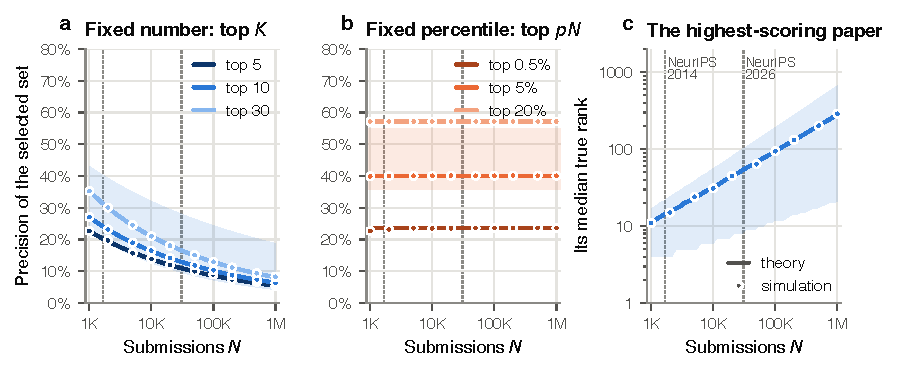
\includegraphics[width=\textwidth]{fig1_main.pdf}
\caption{\textbf{A fixed-number selection loses accuracy as conferences grow; a fixed-percentile one keeps it.} (a) Precision of the top $K$ papers by score: the share truly among the $K$ best. (b) Precision of the top $pN$ papers. (c) Median true rank of the highest-scoring paper. Lines: exact theory at the calibrated reliability $\rho^2=0.50$; bands: $\rho^2=0.44$ to 0.71 (top 10 in a, top 5\% in b); dots: simulation; dotted lines: NeurIPS 2014 and 2026. Top-10 precision falls from 27\% to 6\% and the winner's median rank rises from 11 to 281, while top-$p$ sets hold their precision. Awards and fixed oral slots are the decisions that growth erodes.}
\label{fig:main}
\end{figure}

We ask how the quality of a conference's selections changes as the number of submissions $N$ grows with the process fixed, and which parameters of the review system decide it. A \emph{fixed-number} selection takes the top $K$ papers by score, with $K$ constant in $N$ (awards, a fixed number of talks). A \emph{fixed-percentile} selection takes the top fraction $p$ (acceptance, an oral tier set as a share of submissions). We vary the number of submissions ($10^3$ to $10^6$); the noise model (reviewer noise, noise shared by all handlers of a paper, Gaussian or heavy-tailed); reviews per paper (1 to 50); the scoring function and its discretisation (continuous, 1--10, ICLR's $\{1,3,5,6,8,10\}$, six-point, five-point); the quality distribution (Gaussian, bounded, exponential, lognormal, heavy-tailed); and the acceptance rate (10\% to 40\%). The conclusions, in order of importance:

\begin{enumerate}
\item \textbf{Fixed-number selections degrade as conferences grow; fixed-percentile selections do not} (Fig.~\ref{fig:main}). Top-10 precision falls from 27\% at $N=10^3$ to 6\% at $10^6$.
\item \textbf{The decay is a power law with no floor} (Fig.~\ref{fig:mechanism}), $N^{-(1-\rho)/(1+\rho)}$ up to a logarithm and steeper at real sizes. The best paper is in the top 10 by score 49\% of the time at $N=10^3$ and 13\% at $10^6$.
\item \textbf{In the Gaussian model only the reliability $\rho^2$ of the mean score matters, and it is costly to raise} (Fig.~\ref{fig:parameters}). Holding top-10 precision from $10^3$ to $10^6$ submissions takes 11 reviews per paper instead of 3.
\item \textbf{The tails decide the top} (Fig.~\ref{fig:robustness}). Power-law ($t_3$) quality makes fixed-$K$ selection improve with $N$; bounded quality, heavy-tailed noise or coarse score scales make it collapse.
\item \textbf{The accept/reject boundary is robust and $N$-free} (Fig.~\ref{fig:boundary}). At 25\% acceptance, 39\% of accepted papers are outside the true top 25\% in every variant: about 160 papers at NeurIPS 2014 and 3,050 in 2026.
\item \textbf{The real top tier is noisier than the model} (Fig.~\ref{fig:validation}): a second committee rejected 54\% of NeurIPS 2021 spotlights; the model predicts 31\%.
\end{enumerate}

\section{Methods}

\begin{figure}[t]
\centering
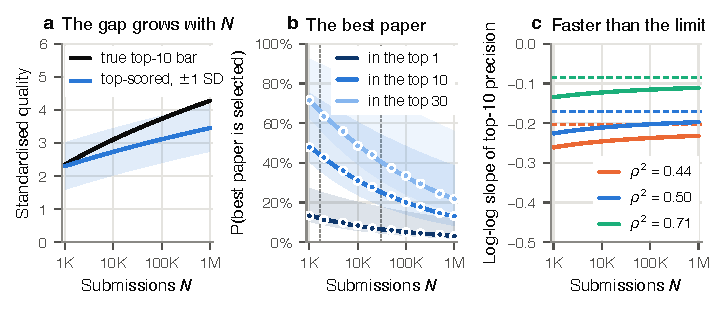
\includegraphics[width=\textwidth]{fig2_mechanism.pdf}
\caption{\textbf{The top-scored papers fall ever further below the quality the true top $K$ requires, so fixed-$K$ precision decays without a floor.} (a) Standardised quality of the 10th-best paper, and of the top-scored paper ($\rho\,\E[S^\ast_{(1)}]$, band $\pm1$ conditional SD); central reliability. (b) Probability that the best paper is in the top $K$ by score; lines theory, dots simulation. (c) Local log-log slope of top-10 precision (solid) and its limit $-(1-\rho)/(1+\rho)$ (dashed). In (a) the bar rises like $\sqrt{2\log N}$, the top-scored paper's quality only $\rho$ times as fast. From $N=10^3$ to $10^6$ the decay is 1.2 to 1.4 times faster than the limit.}
\label{fig:mechanism}
\end{figure}
\begin{figure}[t]
\centering
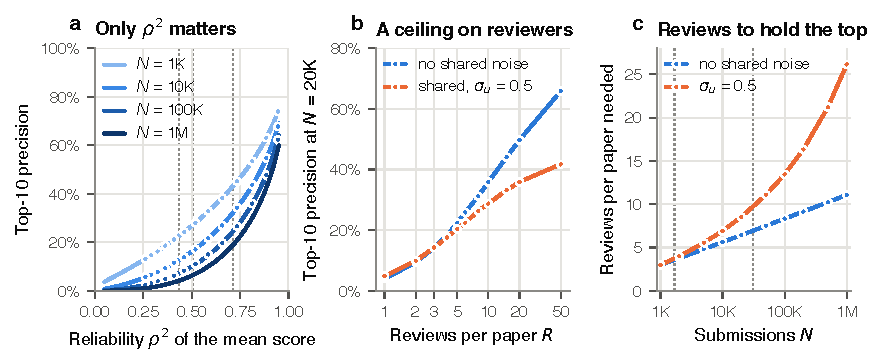
\includegraphics[width=\textwidth]{fig3_parameters.pdf}
\caption{\textbf{Reviewer noise, reviewer count and shared noise act only through the reliability $\rho^2$, and holding the top steady as $N$ grows takes many more reviews.} (a) Top-10 precision against $\rho^2$ at four sizes: theory (lines) and, at the three smaller sizes, simulation over 13 reviewer-noise values at $R=3$ (dots); dotted lines mark the three calibrated levels. (b) Top-10 precision at $N=20{,}000$ against reviews per paper, per-review noise fixed at its $R=3$ calibration, without and with shared noise. (c) Reviews per paper that keep top-10 precision at its $N=10^3$, $R=3$ value. The same reliability buys less at a larger conference, and shared noise caps what extra reviewers can buy.}
\label{fig:parameters}
\end{figure}
\begin{figure}[t]
\centering
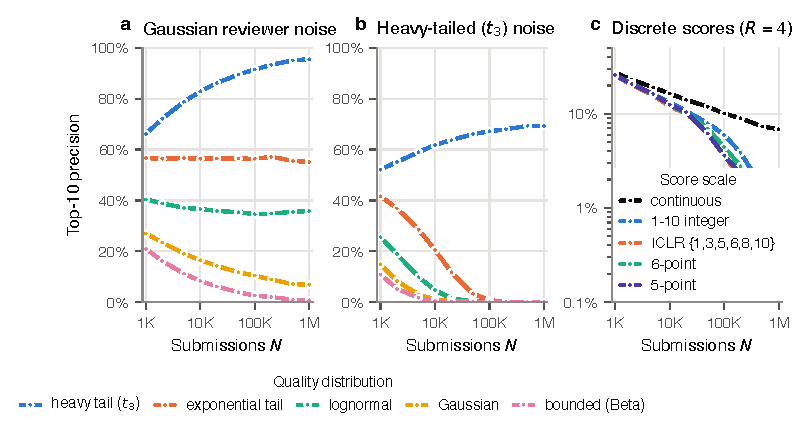
\includegraphics[width=\textwidth]{fig4_robustness.pdf}
\caption{\textbf{Whether the top of the ranking degrades with $N$ depends on the tail of quality relative to the tail of the noise, and coarse score scales speed the collapse.} (a) Top-10 precision for five quality distributions with equal mean and SD, Gaussian reviewer noise, $R=3$, each refitted to the central disagreement. (b) The same with $t_3$ reviewer noise. (c) Top-10 precision (log scale) on five score scales, $R=4$, each refitted; ties broken at random. Power-law ($t_3$) quality spreads the best papers apart, so precision rises; bounded quality or heavy-tailed noise turn the top into a contest of noise. The accept-level data used for calibration cannot tell these cases apart.}
\label{fig:robustness}
\end{figure}
\begin{figure}[t]
\centering
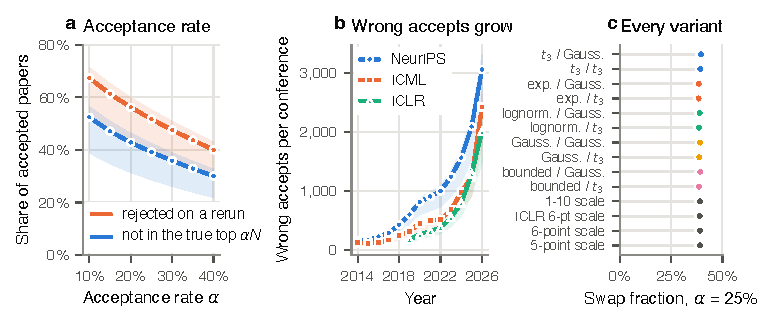
\includegraphics[width=\textwidth]{fig5_boundary.pdf}
\caption{\textbf{At the accept/reject boundary the share of wrong decisions is set by the acceptance rate and the reliability, so their number grows with submissions.} (a) Swap fraction (accepted papers outside the true top $\alpha N$) and two-committee disagreement against the acceptance rate, $N=10^4$; lines theory with pessimistic-to-optimistic bands, dots simulation. (b) Expected wrong accepts at each NeurIPS, ICML and ICLR year's own size and acceptance rate. (c) Swap fraction at 25\% acceptance and $N=10^5$ for every quality/noise pair and score scale, each refitted. Every variant gives 38\% to 40\%: unlike the top of the ranking, this result does not depend on the unknown tails.}
\label{fig:boundary}
\end{figure}
\begin{figure}[t]
\centering
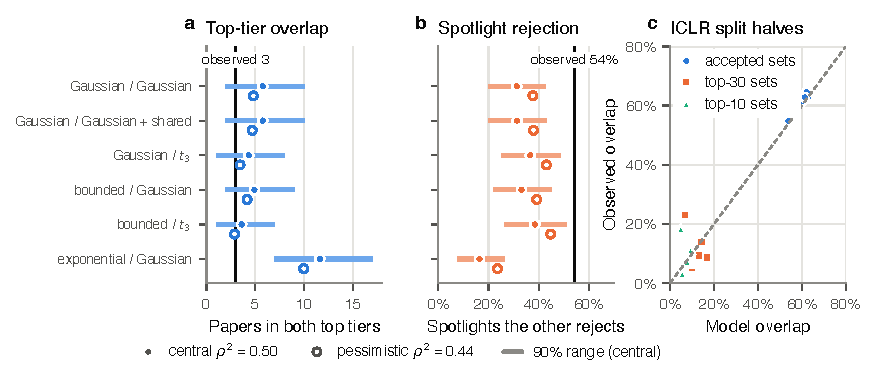
\includegraphics[width=\textwidth]{fig6_validation.pdf}
\caption{\textbf{Data the model was not fitted to show a top tier noisier than the calibrated model, and an accept/reject boundary close to it.} (a) Predicted overlap of the two committees' oral-plus-spotlight tiers (29 and 25 papers) in the NeurIPS 2021 experiment for six variants (quality / noise): mean and 90\% range over 4,000 replays at the central level (filled) and mean at the pessimistic level (open); observed 3. (b) Predicted share of one committee's spotlights rejected by the other; observed 54\%. (c) ICLR 2021--2025 split halves: observed against predicted overlap of the halves' accepted, top-30 and top-10 sets, with reviewer noise fitted to the observed half-mean correlation. At the central level the observed spotlight rejection lies outside every variant's 90\% range, so Fig.~\ref{fig:main}a is, if anything, optimistic.}
\label{fig:validation}
\end{figure}

\paragraph{Model.} A conference receives $N$ papers. Paper $i$ has true quality $q_i\sim\mathcal N(5,1.2^2)$ on a latent 1--10 axis and receives $R$ reviews $s_{ij}=q_i+u_i+\varepsilon_{ij}$, with shared noise $u_i\sim\mathcal N(0,\sigma_u^2)$ and reviewer noise $\varepsilon_{ij}\sim\mathcal N(0,\sigma_\varepsilon^2)$. Shared noise is what every handler of a paper sees alike (area chair, presentation, fashion); more reviewers do not average it out. The score $\bar s_i$ is the mean of the $R$ reviews; ties are broken at random. Discrete variants snap each review to the nearest point of a score scale before averaging. Other variants change the quality distribution (bounded Beta, exponential tail, lognormal, Student-$t_3$), all with the same mean and SD, or make the reviewer noise $t_3$ with the same SD. The reliability of the score is $\rho^2=\operatorname{corr}(\bar s,q)^2=\sigma_q^2/(\sigma_q^2+\sigma_u^2+\sigma_\varepsilon^2/R)$. A second committee redraws $u$ and $\varepsilon$, as the field experiments used disjoint reviewers and area chairs, so the two committees' scores correlate at $\rho^2$.

\paragraph{Metrics.} $\Top_K(q)$ is the set of the $K$ papers of highest true quality. The \emph{precision} of a selection $\Top_K(\bar s)$ is $|\Top_K(\bar s)\cap\Top_K(q)|/K$. With a fixed quota each undeserving paper selected displaces a deserving one, so $1-\text{precision}$ is also the share of deserving papers left out; at the acceptance rate $\alpha$ it is the \emph{swap fraction}. We also report the probability that the truly best paper is in $\Top_K(\bar s)$, the true rank of the top-scored paper, and the two-committee \emph{disagreement} $P(\text{rejected by 2}\mid\text{accepted by 1})$. The share of papers with inconsistent decisions is $2\alpha$ times it.

\paragraph{Calibration.} In the Gaussian model the disagreement at rate $\alpha$ is $1-P_2(z_\alpha,z_\alpha;\rho^2)/\alpha$, with $P_2(a,b;r)$ the standard bivariate normal upper orthant probability and $z_\alpha=\Phi^{-1}(1-\alpha)$. Inverting it gives $\rho^2$ from each experiment. NeurIPS 2021 gives $\rho^2=0.50$: 203 of its 764 decided papers were inconsistent at a mean acceptance rate of 26.2\%. (The often-quoted 23.0\% at 22.7\% gives 0.56 but counts 118 withdrawn papers as agreements.) The NeurIPS 2014 table gives 0.53; the quoted 2014 figure \citep{price2014nips}, which pairs the 25.9\% inconsistency with the committees' 22.5\% target rate (the conference accepted 24.7\%), gives 0.44; the committees' score correlations give 0.55 (2014) and 0.58 to 0.59 (2021). The ICLR correlation of 0.40 between two reviews of a paper \citep{berenslab_iclr} gives 0.71 by Spearman--Brown at 3.7 reviews, an upper bound because it omits noise the reviewers share. We carry three levels: pessimistic $\rho^2=0.44$, central $0.50$, optimistic $0.71$. Each non-Gaussian variant is refitted by bisection on $\sigma_\varepsilon$ so that its simulated disagreement at 26.2\% acceptance equals the Gaussian model's at the same level (5,000 papers, 2,000 conference pairs, common random numbers). On coarse scales, where ties make the disagreement non-monotone in $\sigma_\varepsilon$, we take the root above its minimum.

\paragraph{Analysis and simulation.} For the Gaussian model we compute every metric exactly at finite $N$ as a two-dimensional integral over order statistics of quality and score and their concomitants \citep{yeo1984selection,nagaraja1994concomitants,david2003order}, and derive its large-$N$ law. Two independent derivations were reconciled and checked by quadrature up to $N=10^{300}$. The simulator draws 10,000 conferences per setting up to $N=2\times10^4$, then a budget of $2\times10^8$ paper draws ($10^9$ and at least 2,000 conferences in the main sweep), and 10,000 at every $N$ for the best-paper probability. Theory and simulation agree within Monte Carlo error.

\paragraph{Validation data.} The NeurIPS 2021 report tabulates both committees' recommendations, including orals and spotlights \citep{beygelzimer2023neurips}. Public ICLR reviews \citep{paperlists} let us split each paper's reviews into two halves and treat each half as a committee.

\section{Results}

\paragraph{Fixed number against fixed percentile.} At the central reliability, top-10 precision is 27\% at $N=10^3$, 16\% at $10^4$, 10\% at $10^5$ and 6\% at $10^6$, and top-5 and top-30 precision fall in parallel (Fig.~\ref{fig:main}a). The precision of a fixed share does not move: 24\% for the top 0.5\%, 40\% for the top 5\%, 57\% for the top 20\% (Fig.~\ref{fig:main}b), and 61\% for a 25\% accept set. A set of only $K$ papers loses a relative $c_p/K$ ($c_p=0.12$ at $p=25\%$, rising to $\rho/(1+\rho)^2=0.24$ as $p\to0$), so the five papers of the top 0.5\% at $N=10^3$ reach 23\%. A random paper's score and quality have the same joint law at any $N$, so the share above two fixed quantiles is fixed at $P_2(z_p,z_p;\rho)/p$; a fixed $K$ is a shrinking share $K/N$ that reaches ever further into the tail. The selected papers stay very good: the top 10 by score sit, on average, at the 97th true percentile at $N=10^4$ and the 99.5th at $10^6$, and the share inside the true top 1\% rises from 53\% to 88\%. They are rarely the best. The median true rank of the highest-scoring paper is 11 at $N=10^3$ and 281 at $10^6$ (Fig.~\ref{fig:main}c).

\paragraph{Why fixed-$K$ precision decays.} Write $Q^\ast$ and $S^\ast$ for standardised quality and score, a bivariate normal pair with correlation $\rho$. The $K$ best qualities and the $K$ best scores both lie near $b_N=\Phi^{-1}(1-1/N)\approx\sqrt{2\log N}$. A paper with score $s$ has quality $\mathcal N(\rho s,1-\rho^2)$. So the top-scored papers fall short of the true top-$K$ bar by about $(1-\rho)b_N$, a gap that grows with $N$, while the spread $\sqrt{1-\rho^2}$ does not (Fig.~\ref{fig:mechanism}a). The large-$N$ law is
\begin{equation}
\text{prec}_{N,K}\sim\frac{(1+\rho)^2}{K\sqrt{1-\rho^2}}\left[\frac{\Gamma\!\left(K+\frac{1}{1+\rho}\right)}{\Gamma(K)}\right]^2 N^{-\frac{1-\rho}{1+\rho}}\,(4\pi\log N)^{-\frac{\rho}{1+\rho}},
\end{equation}
with a relative correction of order $\log\log N/\log N$. The limit is zero for every $\rho<1$. The exponent is 0.17 at the central reliability (0.20 pessimistic, 0.08 optimistic). The correction is still large at real sizes: between $N=10^3$ and $10^6$, top-10 precision falls as $N^{-0.21}$ at the central level, 1.23 times faster than the limit (Fig.~\ref{fig:mechanism}c). Placing the selected papers at the score threshold gives the right exponent but a constant too small by $(1+\rho)R_K$, because selected scores lie above the threshold and the $K$-th order statistics fluctuate ($R_K=[\Gamma(K+c)/(\Gamma(K)K^c)]^2$, $c=1/(1+\rho)$). The probability that the best paper is in the top $K$ decays at the same rate (Fig.~\ref{fig:mechanism}b): from 49\% to 13\% for $K=10$, and from 14\% to 3\% for $K=1$. The overlap of two committees' top 10, which an experiment could observe, decays faster, as $N^{-(1-\rho^2)/(1+\rho^2)}$: from 13\% at $N=10^3$ to 1\% at $10^6$.

\paragraph{The review-system parameters.} In the Gaussian model every metric depends on $\sigma_\varepsilon$, $R$ and $\sigma_u$ only through $\rho^2$ (Fig.~\ref{fig:parameters}a). More reviewers raise $\rho^2$, but shared noise caps it at $\sigma_q^2/(\sigma_q^2+\sigma_u^2)$, which is 0.85 for $\sigma_u=0.5$. With both variants fitted to the data at $R=3$, raising $R$ from 3 to 10 at $N=20{,}000$ lifts top-10 precision from 14\% to 36\% without shared noise and to 29\% with it (Fig.~\ref{fig:parameters}b). Keeping top-10 precision at its $N=10^3$ value takes 5.6, 8.3 and 11.1 reviews per paper at $N=10^4$, $10^5$ and $10^6$, or 6.9, 13.4 and 26.1 with shared noise (Fig.~\ref{fig:parameters}c). Real conferences kept three to four.

\paragraph{The tails decide the top.} At equal mean, SD and disagreement, the shape of the quality distribution changes fixed-$K$ precision completely (Fig.~\ref{fig:robustness}a). The rule compares the top quality gaps with the noise: precision tends to zero when the noise tail is heavier or the gaps shrink, levels off when they stay fixed, and tends to one when they grow. From $N=10^3$ to $10^6$, top-10 precision falls from 27\% to 6\% for Gaussian quality and from 21\% to 0.7\% for bounded quality, whose best papers crowd against the bound where noise sorts them. It stays near 56\% for exponential quality, whose top gaps stay of order $\sigma_q$, drifts from 40\% to 36\% for lognormal quality, whose gaps grow too slowly to help in range, and rises from 66\% to 96\% for $t_3$ quality, whose top gaps grow like $N^{1/3}$. Heavy-tailed reviewer noise makes all but the last collapse (Fig.~\ref{fig:robustness}b): outlier reviews then dominate the top scores, and precision falls toward the chance level $K/N$, unless quality is equally heavy-tailed, in which case it levels off near 69\%. Fixed-percentile precision does not depend on $N$ for any shape.

\paragraph{Score scales.} With $R=4$ and each scale refitted, discretisation costs little at small $N$ and much at large $N$ (Fig.~\ref{fig:robustness}c). At $N=10^4$, top-10 precision is 16\% with continuous scores and 12\% to 13\% on every discrete scale; at $10^6$ it is 6\% against 0.6\% to 1.2\%. At large $N$ many papers share the highest attainable mean score, and random tie-breaking makes the selection a lottery inside that class, so precision eventually falls as $1/N$. The 1--10 scale holds up best; the five-point and ICLR six-point scales do worst. Random tie-breaking models an area chair with no information, continuous scores one with full information. Fixed-percentile precision changes by at most 3 points, and the 25\% swap fraction by under 0.2. Shifting the latent mean by half a scale step changes top-10 precision at $N=10^5$ by up to a factor of three.

\paragraph{The accept/reject boundary.} The swap fraction depends on $\alpha$ and $\rho^2$ but not on $N$. At the central reliability it is 52\% at 10\% acceptance, 43\% at 20\%, 39\% at 25\% and 30\% at 40\% (Fig.~\ref{fig:boundary}a). It falls as $\alpha$ rises because wrong accepts per paper, $\alpha$ times the swap fraction, are zero at $\alpha=0$ and concave in $\alpha$. The two-committee disagreement has the same form at correlation $\rho^2$ and is larger: 52\% at 25\% acceptance. Wrong accepts number the swap fraction times $\alpha N$, so they grow with submissions: about 160 at NeurIPS 2014 and 3,050 at NeurIPS 2026, and about 2,420 at ICML and 2,010 at ICLR in 2026 (Fig.~\ref{fig:boundary}b; 1,640 on ICLR's decided papers). Across all ten quality-and-noise pairs and all scales, the swap fraction at 25\% acceptance lies between 38.4\% and 39.6\% (Fig.~\ref{fig:boundary}c), because each variant is fitted to the same accept-level disagreement.

\paragraph{Out-of-sample tests.} The calibration uses only the accept-level disagreement, so the NeurIPS 2021 top tier is a test. Among the 764 decided papers, the two committees' oral-plus-spotlight tiers held 29 and 25 papers and shared 3, and of each committee's spotlights the other rejected 13 (of 25 and of 23), 26 of 48 in all (54\%). We replayed the experiment in six calibrated variants, as a random 764-paper subsample of a 7,902-paper conference (Fig.~\ref{fig:validation}a,b). At the central level the Gaussian model predicts a tier overlap of 5.8 papers (90\% range 2 to 10; $P(\le3)=0.17$) and 31\% of spotlights rejected ($P(\ge54\%)=0.002$). Shared noise changes nothing, as theory requires. The two variants with heavy-tailed noise come closest (overlap 3.6 to 4.3; 37\% to 39\% rejected), and reach 43\% to 45\% at the pessimistic level, where the observed 54\% lies inside their 90\% ranges ($P(\ge54\%)=0.07$ and $0.11$). Exponential-tail quality fails (overlap 11.6), and so does the optimistic reliability in every variant. The real top tier is therefore noisier than the calibrated model, and the variants that fit it best are those in which fixed-$K$ precision decays fastest. Part of the excess is by design: the 2021 top tier used criteria beyond reviewer scores, such as broad interest.

For ICLR 2021--2025 we split the reviews of each decided paper with at least four reviews into two halves of two, re-made the decisions in each half at the observed acceptance rate, and fitted reviewer noise to the observed half-mean correlation (0.49 to 0.55). The model then reproduces the share of inconsistent decisions (29\% to 33\% against 29\% to 32\% observed) and the overlap of the two accepted sets (54\% to 63\% against 55\% to 65\%). Top-10 and top-30 overlaps are small in both and close in 2021, but the observed values are 50\% to 92\% of the model's in 2022--2024 and 3.5 to 3.9 times it in 2025 (Fig.~\ref{fig:validation}c). The halves share the area chair and the rebuttal, so this test favours consistency.

\paragraph{Limitations.} Quality is one-dimensional and drawn from one fixed distribution at every $N$; reviewers are exchangeable, with no leniency offsets or reviewer matching; the area chair appears only as shared noise; there is no rebuttal, discussion, strategic behaviour, desk rejection or withdrawal; and decisions use the mean score alone. The calibration rests on two experiments of 166 and 764 decided papers, whose sampling error covers much of the range between our pessimistic and optimistic levels. The tails of the quality and noise distributions, which decide the top-of-ranking results, are not identified by accept-level data.

\bibliographystyle{plainnat}
\footnotesize
\bibliography{refs}

\end{document}
